\section{Implementation}
	\subsection{Sprint 0}
		\subsubsection{Sprint Planning}
		As the initial sprint of the project this sprint was concerned with setting up and configuring CI/CD tools for the project. The main tool of the CI/CD process considered were a Jenkins build server to continuously build and deploy the code and SonarQube to test code coverage and quality. Given the agile developments methodology was important to implement these steps early in the project and therefore they were undertaken during the initial sprint.

		\subsubsection{Sprint Review}
		The following goals were achieved:
		\begin{itemize}
			\item A Jenkins build server was deployed to AWS;
			\item An AWS ECS instance to run the web app was deployed;
			\item A skeleton React app was created with a defined Dockerfile to build image of the app;
			\item A Jenkins pipeline was created to build the image of the app and deploy it to AWS on every commit to GitHub;
			\item On account on SonarCloud was created, a cloud based service of SonarQube. 
		\end{itemize}
		
		\subsubsection{Sprint Retrospective}
		\textbf{What did we do well?}
		\begin{itemize}	
			\item CI/CD process has been set-up and implemented.
		\end{itemize}
		
		\noindent\textbf{What could have been done better?}
		\begin{itemize}
			\item Story Points have not been allocated to tickets;
			\item Breakdown of backlog could be improved, better utilising Epics, Issues and Subtasks.
		\end{itemize}
		
		\noindent\textbf{Actions}
		\begin{itemize}
			\item Rob Shelly to further refine the product backlog;
			\item Rob Shelly to add story points to tickets on backlog.
		\end{itemize}
		
		\subsubsection{Personal Reflection}
		This sprint highlighted the need for story points as the lack of such has meant there is not burndown chart for the sprint. Adding story points along with a well refined and organised backlog will allow for better sprint planning in the future.

	\subsection{Sprint 1}
		\subsubsection{Sprint Planning}
		The planning around for this session was based on the existing Jenkins Jobs created during the prototyping process. These jobs need to exist on the Jenkins server when the system is initially deployed/installed by a user. I.e, the user does not create these jobs.
		Therefore, these jobs need to be created during the installation process. This sprint focused on creating \textit{yaml} files for these jobs which can be used by \textit{Jenkins Job Builder} (JJB) to create the jobs during set-up. This also provided the ability to quickly recreate the jobs should the Jenkins Server crash during development.

		\subsubsection{Sprint Review}
		The \textit{yaml} files were created and tested for the following Jenkins jobs:
		\begin{itemize}
			\item Deploy: Spins up a restoration server in AWS (i.e. a server with the correct DBMS installed)
			\item Decrypt:  Moves a backup file to a restoration server and decrypts it.
			\item Restore: Imports a backup file into the DBMS and performs a read of the data.
			\item Destroy: Destroys the restoration server after a successful backup restoration.
			\item Backup Restoration Pipeline:	Performs a full backup test restoration (using the above Jenkins jobs).
		\end{itemize}
		The sprint delivered on it's main focus of creating the \textit{yaml} files. However, further tickets which would have built upon the prototype (displaying the result of the restoration) were not completed.

		\subsubsection{Sprint Retrospective}
		\textbf{What did we do well?}
		\begin{itemize}	
			\item Technically mastered the complexity of the project, have a
			vision and a direction to move towards;
			\item Backlog is very mature, the Minimum Viable Product (MVP) is almost visible;
			\item JJB was utilised and I now understand how Jenkins jobs
			work;
			\item Story Points were introduced and helped to guide the work.
		\end{itemize}
		
		\noindent\textbf{What could have been done better?}
		\begin{itemize}
			\item Burndown was inconsistent as most of the work was completed within a short period of time during the sprint;
			\item Domain knowledge in certain areas (JJB) was not as strong
			as I would have liked it to be, which slowed me down and
			was not reflective of the complexity I had awarded those
			tickets;
			\item Outward communication to the stakeholders (Leigh \& Paul)
			was not as good as it could have been.
		\end{itemize}

		\noindent\textbf{Actions}
		\begin{itemize}
			\item Rob Shelly to get a draft of wireframes to Leigh by next Monday;
			\item Rob Shelly to complete MVP plan for the backend system and include an API definition and CLI guide;
      \item Rob Shelly to send regular updates on progress to stakeholders.
		\end{itemize}

		\subsubsection{Sprint Burndown}
		
 		\begin{figure}[H]
      \setlength{\belowcaptionskip}{15pt plus 3pt minus 2pt}
      \caption{Sprint 1 Burndown Chart}
      \centering
      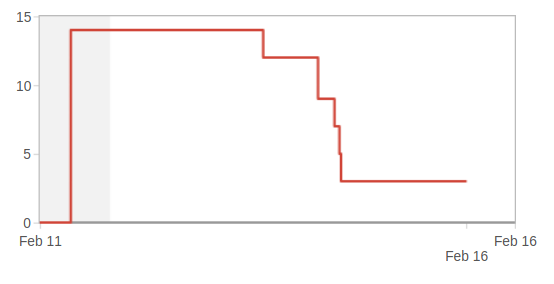
\includegraphics[width=\textwidth,keepaspectratio]{burndown-sprint-1}
      \label{fig:burndown-sprint-1}
    \end{figure}
   
		\subsubsection{Personal Reflection}
		I was happy with the progress of this sprint as I felt creating the \textit{yaml} files for the Jenkins jobs was an vital task, not only to enable an MVP to be packaged as a deployable system, but to provided an easy method of recreating the Jenkins jobs should there be a loss of AWS servers during development.
		
		This sprint also highlighted the importance of planning the sprint with respect to other college work to be completed in the given time frame. Although, this sprint was planned for two weeks, the entirety of the work was completed within a number of days during the later of two weeks. In future, if other college work will take precedence for a number of days, I may plan to delay beginning the sprint, allowing the final burndown chart to better reflect the progress of work over the sprint.
    
  \subsection{Sprint 2}
  \subsubsection{Sprint Planning}
  Planning for this sprint focused on completing the API for my systems. Through conversations with the stakeholders it was decided that the priority for this sprint should be completing the API and it's documentation. Creating the web app frontend for the API could be completed later. However, given that there was still quite a larger number of API related tickets on the product backlog, not all were rough into this sprint.
  
  \subsubsection{Sprint Review}
  The following API function were implemented:
  \begin{itemize}
    \item Fetch results of all recent test restoration;
    \item Fetch a list of all scheduled test restorations;
    \item Create a new test restoration schedule;
    \item Update test restoration schedule;
    \item Delete a test restorations schedule;
    \item Fetch results of all test restorations for a given schedule;
    \item Add an SSH key to the system;
    \item Add a GPG key to the system.
  \end{itemize}
  Documentation for each of the API functions was also completed using Swagger Docs. Thus, the sprint delivered on it's goal of completing and documenting the bulk of the API functions.
  
  \subsubsection{Sprint Retrospective}
  \textbf{What did we do well?}
  \begin{itemize}
    \item Working on a concentrated area (API) was very beneficial;
    \item Product owners were satisfied with the increase in progress updates;
    \item A lot of knowledge around the documentation using Swagger,  helping to develop the backend without the need for a frontend to test it;
    \item Time management was better than the previous sprint, results on all tickets being completed.
  \end{itemize}
  
  \noindent\textbf{What could have been done better?}
  \begin{itemize}
    \item Burndown chart, although better than the previous sprint is still somewhat inconsistent. However, with all tickets completed, the overall result if still good.
  \end{itemize}
  
  \noindent\textbf{Actions}
  \begin{itemize}
    \item Rob Shelly to complete the last few API related tickets from the backlog in order to allows work to proceed to focus soley on the UI.
  \end{itemize}
  
  \subsubsection{Sprint Burndown}
  
  \begin{figure}[H]
    \setlength{\belowcaptionskip}{15pt plus 3pt minus 2pt}
    \caption{Sprint 2 Burndown Chart}
    \centering
    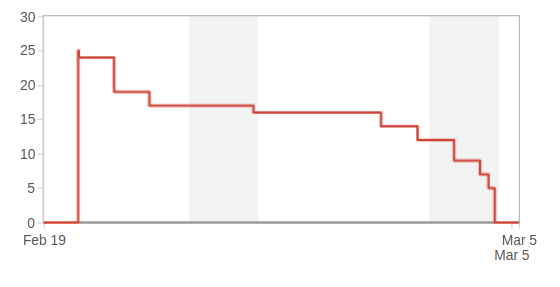
\includegraphics[width=\textwidth,keepaspectratio]{burndown-sprint-2}
    \label{fig:burndown-sprint-2}
  \end{figure}
  
  \subsubsection{Personal Reflection}
  I was very happy with the work completed during this sprint. Prior to Sprint planning and backlog refinement I had been planning on completing tickets by grouping API functions with their corresponding UI elements. However, at the advice of the product owners I decided to focus solely on completing the API first before moving on the the UI.
  
  Having completed the sprint I now feel that separating the API and UI was a much more productive approach. Swagger, which was used to document the API also contains a feature to test the the documented API calls. Therefore, by focusing only on writing and documenting the API, I was able to stay in the mindset of the API functions without having to constantly transition between developing API calls and UI elements, while still being able to test the functions using Swagger.
  
   

	\subsection{Sprint n}

	\subsection{Sprint Metrics}
	% TODO
	TODO

	